\section{Continuous Electron Beam Accelerator Facility}\label{sec:cebaf.desc}

\abbr{CEBAF} utilizes superconducting radio-frequency (\abbr{srf}\label{abbr:srf}) cavities to accelerate electrons and provide a continuous wave beam with 75\% polarization to the three halls simultaneously. A list of some specifications for \abbr{CEBAF} can be found in Table~\ref{tab:cebafspecs}.
%Niobium (\abbrlc{N}{b}\label{abbr:nb}), in a cryogenic system, provides the superconducting environment necessary for \abbr{CEBAF} to obtain a 100\% duty factor because superconducting cavities are non-resistive. Prior to the implementation of \abbr{srf}, copper \abbr{RF}\label{abbr:rf} cavities were used, however due to the resistive properties of copper significant cooling time was needed due to heat produced in the cavity.
\begin{table}
\begin{minipage}{\textwidth}
\begin{center}
\begin{singlespacing}

\caption[\abbr{CEBAF} Operating Specifications]{\label{tab:cebafspecs}Operating specifications of \abbr{CEBAF} at \abbr{JLab}.\cite{cebaf}}

\begin{tabular}{c|c}

%\hline \hline
%
%operation & \multicolumn{3}{c}{Generation} \\
%charge & I & II & III \\


\hline

$\textrm{E}_{min}$ & 0.6 GeV \\
$\textrm{E}_{max}$ & 6.0 GeV \\
$\textrm{I}_{max}$ & 200 $\mu$A \\
Polarization & $\textgreater$ 75\% \\
Geometric emittance & $\textless \ 10^{9}$ m rad \\
Momentum Spread & $10^{-5}$ \\
Average currents (Halls A and C) & 1-150$\mu$A \\
Average currents (Hall B) & 1-100nA \\
Bunch charge & $\textless$ pC \\
Repetition rat & 499 MHz/hall \\ 
Beam size (rms transverse) & $\sim$ 80 $\mu$m \\
Bunch length (rms) & 300 fs, 90 $\mu$m \\
Energy spread & 2.5 x 10$^5$ \\
Beam power & $\textless$ \ MW  \\
Beam loss & $\textless \mu$A  \\
Number of passes & 5 \\
Number of accelerating cavities & 338 \\
Fundamental mode frequency & 1947 MHz \\
Accelerating cavity effective length & 0.5m \\
Cells/cavity  & 5\\
Average $Q_{0}$  & 4.0 x 10$^9$ \\
Implemented $Q_{ext}$  & 5.6 x 10$^6$ \\
Cavity impedance (r/Q)  & 980 $\Omega$ \\
Average cavity accelerating gradient  & 7.5 MV/m \\
RF power  & $\textless$ \ 3.5 kW/cavity \\
Amplitude control  & 1.00 x 10$^{-4}$ rms \\
Phase control  & 0.1$^\circ$ rms \\
Cavity operating temperature  &  2.08 K\\
Heat load @ 2 K  &  $\textless$ 9 W/cavity\\
Liquefier 2 k cooling power  & 5kW \\
Liquefier operating power  &  5MW\\




\hline \hline

\end{tabular}

\end{singlespacing}
\end{center}
\end{minipage}
\end{table}
\vspace{20pt} 

To achieve the running conditions described in Table~\ref{tab:cebafspecs} \abbr{CEBAF} uses a GaAs photocathode laser driven injector system to produce a highly polarized electron beam. The laser pulses create three electron bunches that are bunched together in 2 ns groups, about 90 $\mu$m in length. Each bunch is 499~MHz at the source at 100 keV, spaced apart by 120$^\circ$ of \abbr{rf} phase. Together the electron bunches form a 1497 MHz beam that then enters two 1/4 \abbr{srf} cavities which accelerate the electrons to $\sim$1\% of the total machine energy before it is injected into the \abbr{CEBAF}'s main accelerator. 

When the electron bunches enter the \abbrlc{N}{b} \abbr{srf} cavity, they undergo an acceleration gradient provided by \abbr{rf} standing wave established inside of the cavity. The standing waves are kept in phase with the electron bunches resulting in a continuous positive electric force on each bunch as it passed through a cavity, see Fig.~\ref{fig:jlab.accel}

\begin{figure}\begin{center}
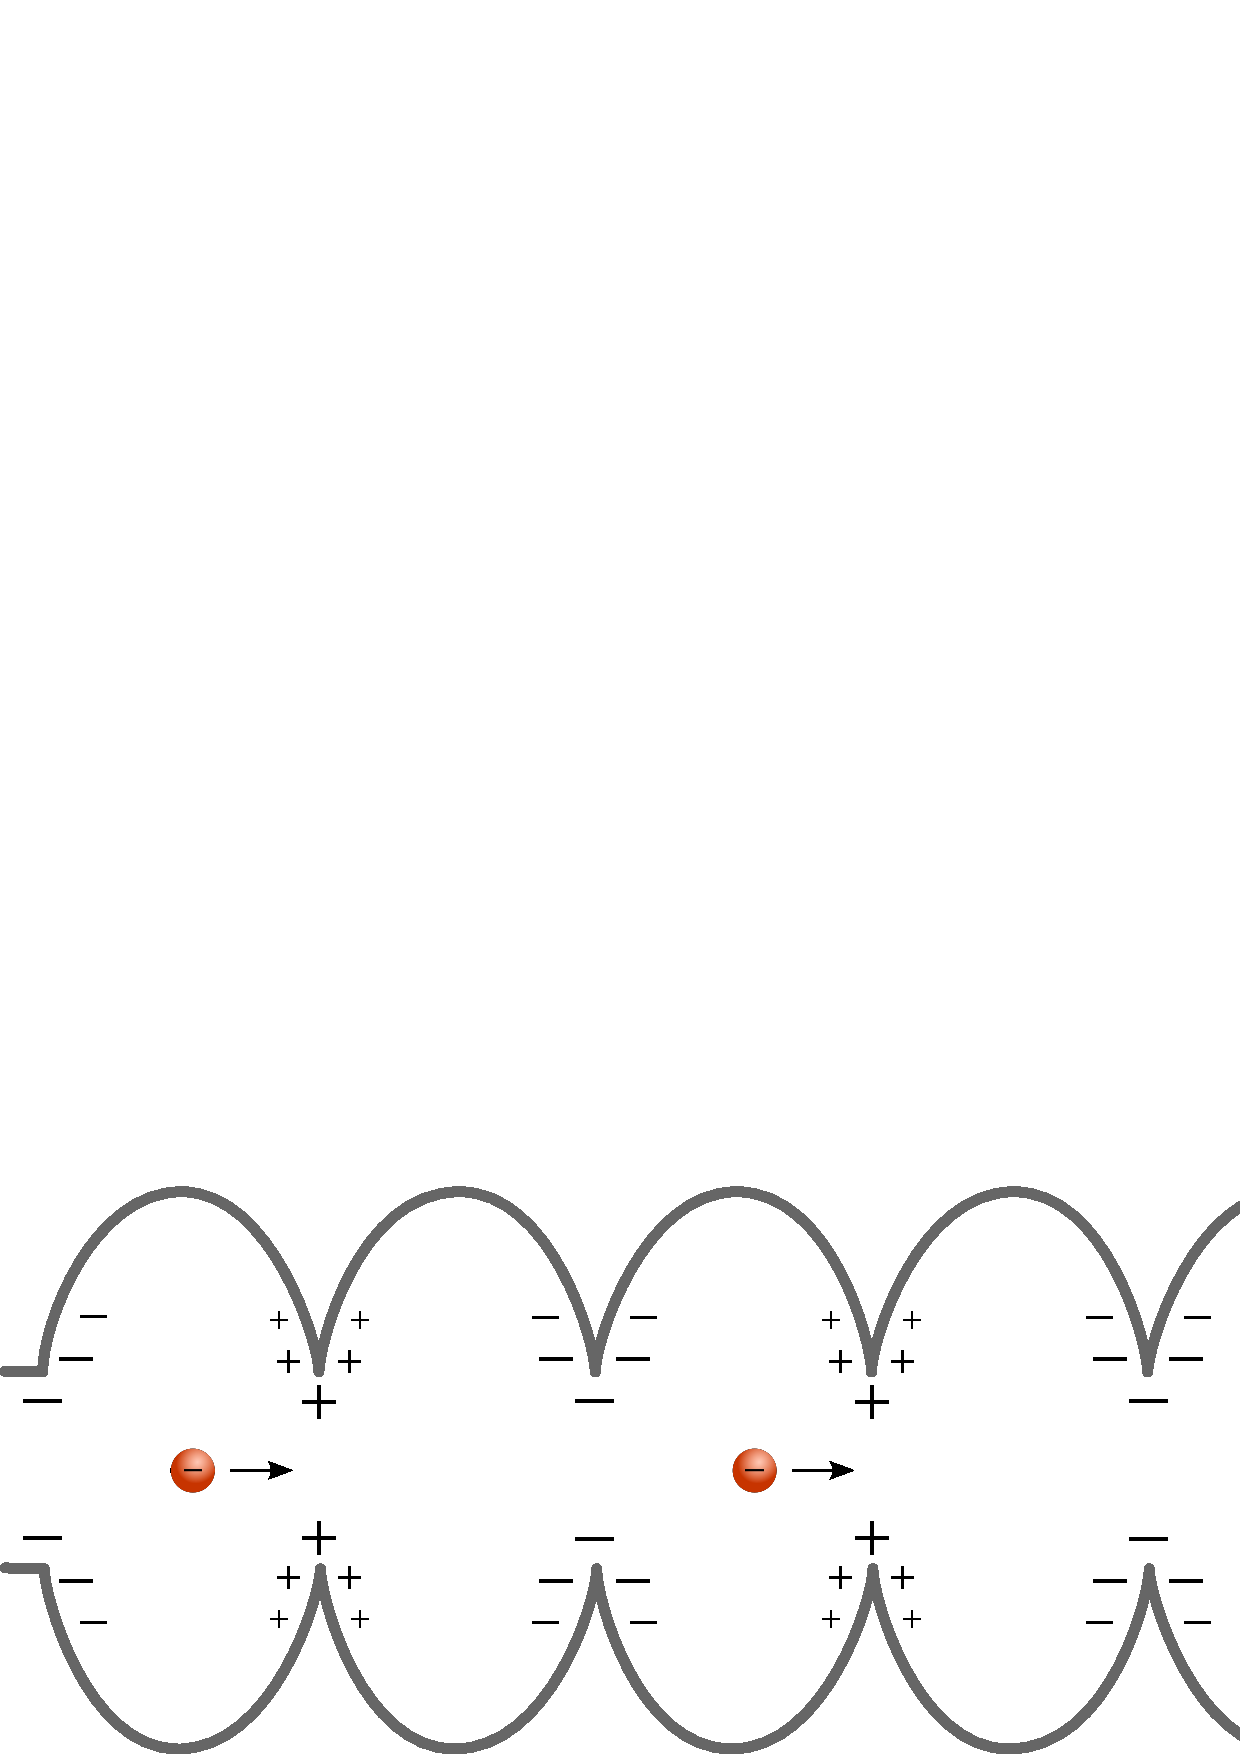
\includegraphics[width=0.8\figwidth,height=\qfigheight]{\grpath/jlab/accelerating_diagram.pdf}
\caption[Accelerating Cavity Diagram]{\label{fig:jlab.accel}Accelerating Cavity Diagram. Electron clusters experience a continuous acceleration due to a standing electromagnetic wave indicated by the positive and negative signs along the inner wall.}
\end{center}\end{figure}

The main accelerator, Fig.~\ref{fig:jlab.cebaf}, consists of a pair of linear accelerators (\abbr{LINAC}s\label{abbr:linac}). Each \abbr{LINAC} contains 168 \abbr{srf} \abbrlc{N}{b} cavities that are submerged in liquid Helium and cooled to 2.08 K, the temperature by which \abbrlc{N}{b} becomes superconducting. In total there are twenty cryogenic modules, each containing eight superconducting niobium cavities as depicted. in Fig.~\ref{fig:jlab.cavity}. 
%The significant cooling requirements are satisfied by the Lab's Central Helium Liquefier (\abbr{CHL}\label{abbr:chl}). 


\begin{figure}\begin{center} 
\includegraphics[width=\figwidth, height=\qfigheight]{\grpath/jlab/niobium_cavity_pair.pdf}
\caption[A \abbr{CEBAF} superconducting niobium cavity pair]{\label{fig:jlab.cavity}A \abbr{CEBAF} superconducting niobium cavity pair. Image Source: \cite{cebaf}}
\end{center}\end{figure}

The beam, once inside the \abbr{LINAC} can be passed up to five times. The \abbr{LINAC}s are connected by two sets of 180$^\circ$ magnetic-dipole bending arcs (see Fig.~\ref{fig:jlab.cebaf}) with a radius of 80~meters. The beam is sent through both accelerators and is then recirculated up to four more times. Each \abbr{LINAC} is capable of accelerating the beam by up to 600~MeV giving approximately 1.2~GeV per pass. Each hall can choose to extract the beam after any number of passes, however the fifth (final) pass can be sent to all three halls simultaneously. It should be noted that although each hall can receive the fifth pass, no two halls can run with the same lower energy \cite{clas.pass}. At the time of the \g12 experiment, the accelerator was capable of delivering a maximum electron beam energy of 5.714~GeV.
%\FloatBarrier